\documentclass[letterpaper,12pt]{article}
\usepackage{amsmath}  % improve math presentation
\usepackage{graphicx} % takes care of graphic including machinery
\usepackage{mathrsfs}


\usepackage[final]{hyperref} % adds hyper links inside the generated pdf file
\hypersetup{
	colorlinks=true,       % false: boxed links; true: colored links
	linkcolor=blue,        % color of internal links
	citecolor=blue,        % color of links to bibliography
	filecolor=magenta,     % color of file links
	urlcolor=blue         
}

\title{Fifth Assignment for Computational Physics}
\date{\today}
\author{Xinyu Liu}


\begin{document}
\maketitle
\tableofcontents

\newpage

\section{My Github Page URL}
\url{https://github.com/rising1227/phys-ga2000}

\section{Problem 1: Exercise 5.15 of Newman}

The Associated Code for this part is ps5-1.py.

We made a function $f(x) = 1 + 0.5* \tanh(2x)$ in the program and find both the analytical derivative$f'(x) = \frac{1}{np.cosh(2x)^2}$ and numerical derivative of that function. The result is plotted as follows:

\begin{table}[!h]
    \centering
    \caption{Numerical and analytical derivative of a function}
    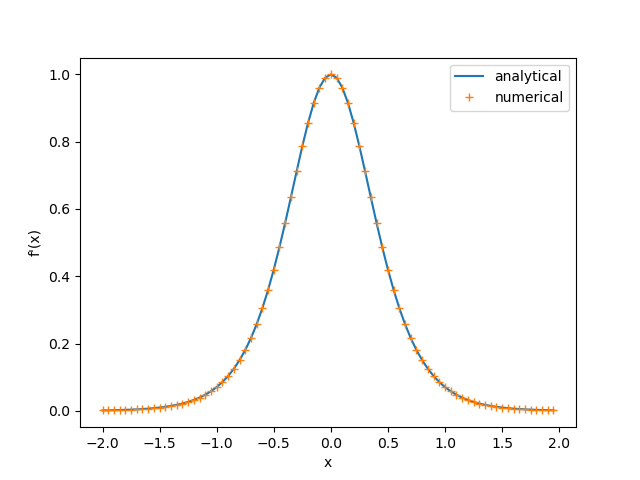
\includegraphics[width=12cm]{ps5-1-1.png}
\end{table}%

We also tried the python package jax to calculate the derivative. It work exactly as advertised:

\begin{table}[!h]
    \centering
    \caption{Numerical and jax derivative of a function}
    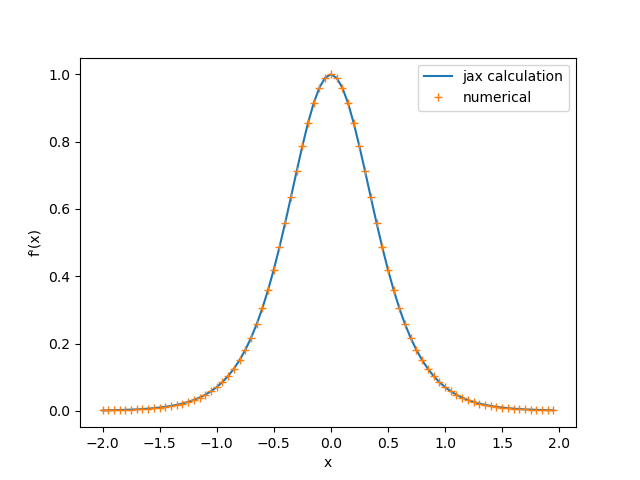
\includegraphics[width=12cm]{ps5-1-2.png}
\end{table}%

\section{Problem 2: Exercise 5.17 of Newman, Gamma function}

The Associated Code for this part is ps5-2.py.

We do exactly expected from the problem. First we plotted the integrand inside Gamma function with a = 2, 3, 4.

\begin{table}[!h]
    \centering
    \caption{Integrand for Gamma function with different a}
    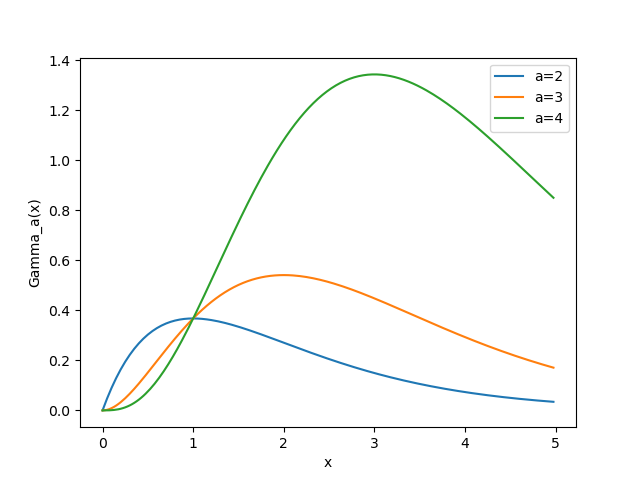
\includegraphics[width=12cm]{ps5-2-1.png}
\end{table}%

\newpage

With $f(x) = x^{a-1} e^{-x}$, the derivative of this function is:

\begin{equation}
    f'(x) = (a-1) x^{a-2} e^{-x} - x^{a-1} e^{-x} = (a-1 - x) x^{a-2} e^{-x}
\end{equation}

So when $x = a-1$, the derivative is 0 and the function takes its maximum value.

Then we do the mapping from infinite integration range to (0,1). For different a, we choose the mapping function to be:

\begin{equation}
    g(x) = \frac{x}{(a-1) + x}
\end{equation}

Also to avoid doing multiplication between very large and small number, we use the formula:

\begin{equation}
    x^{a-1} = e^{(a-1)\ln(x)}
\end{equation}

So that the integrand for Gamma function becomes:

\begin{equation}
    e^{(a-1)\ln(x) - x}
\end{equation}

This is helpful because either $ x^{a-1}$ will be extremely large and $e^{-x}$ will be extremely small for large x, thus inducing large computation error.

After proper change of expression and mapping the integration range, the final integration we'll do is:

\begin{equation}
    \int_{0}^{1} \frac{a-1}{(1-x)^2} * e^{-(a-1)*x/(1-x) + (a-1)*\ln((a-1)*x/(1-x))} dx
\end{equation}

We use gaussian quadrature to numerically evaluate this integral. The integration result is the same as expected:

Calculation of Gamma[1.5] is 0.8862269613087213

Calculation of Gamma[3] is 2.0000000000000004

Calculation of Gamma[6] is 119.99999999999999

Calculation of Gamma[10] is 362879.9999999999



\section{Problem 3: SVD for data fitting}

The Associated Code for this part is ps5-3.py.

We extract the signal data and time and first plot it out:

\begin{table}[!h]
    \centering
    \caption{Signal data against time}
    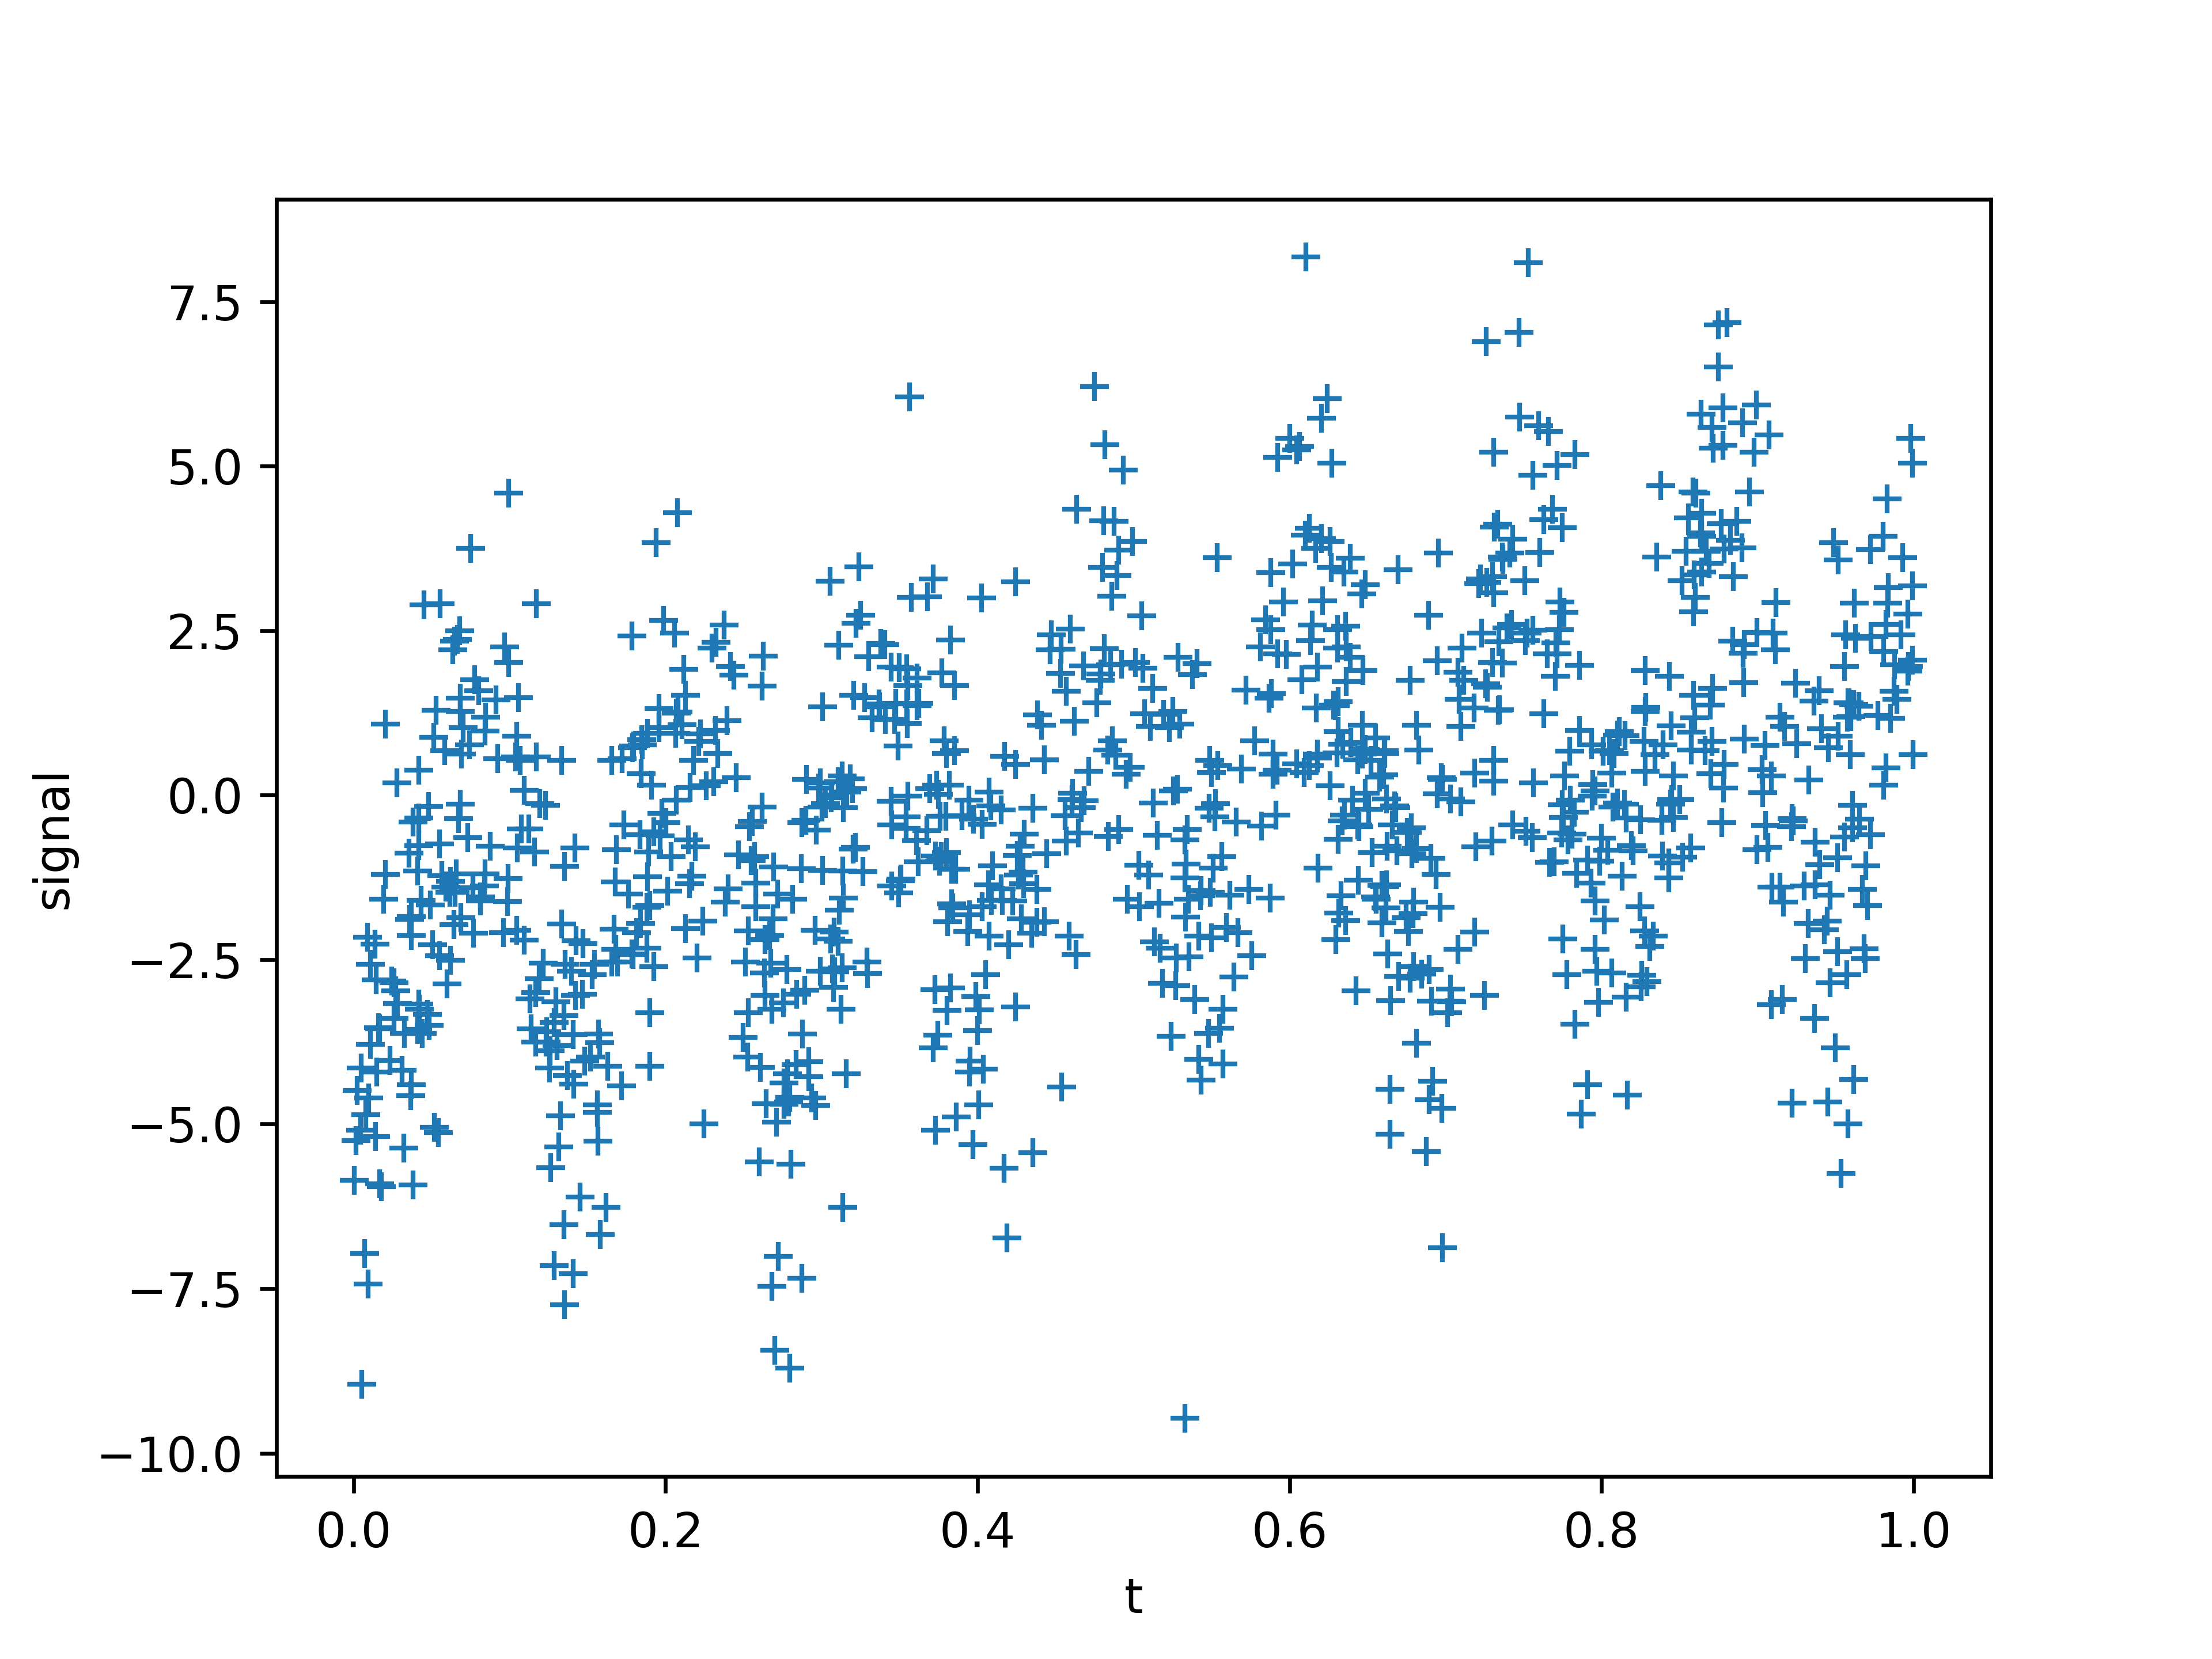
\includegraphics[width=11cm]{ps5-3-1.png}
\end{table}%

In order to avoid calculating very large number, we first rescale the time data by $t' = t*10^{-9}$. Then, we use SVD to fit the data to third-order polynomial. Here's our result:

\begin{table}[!h]
    \centering
    \caption{Fitted signal data to third-order polynomial}
    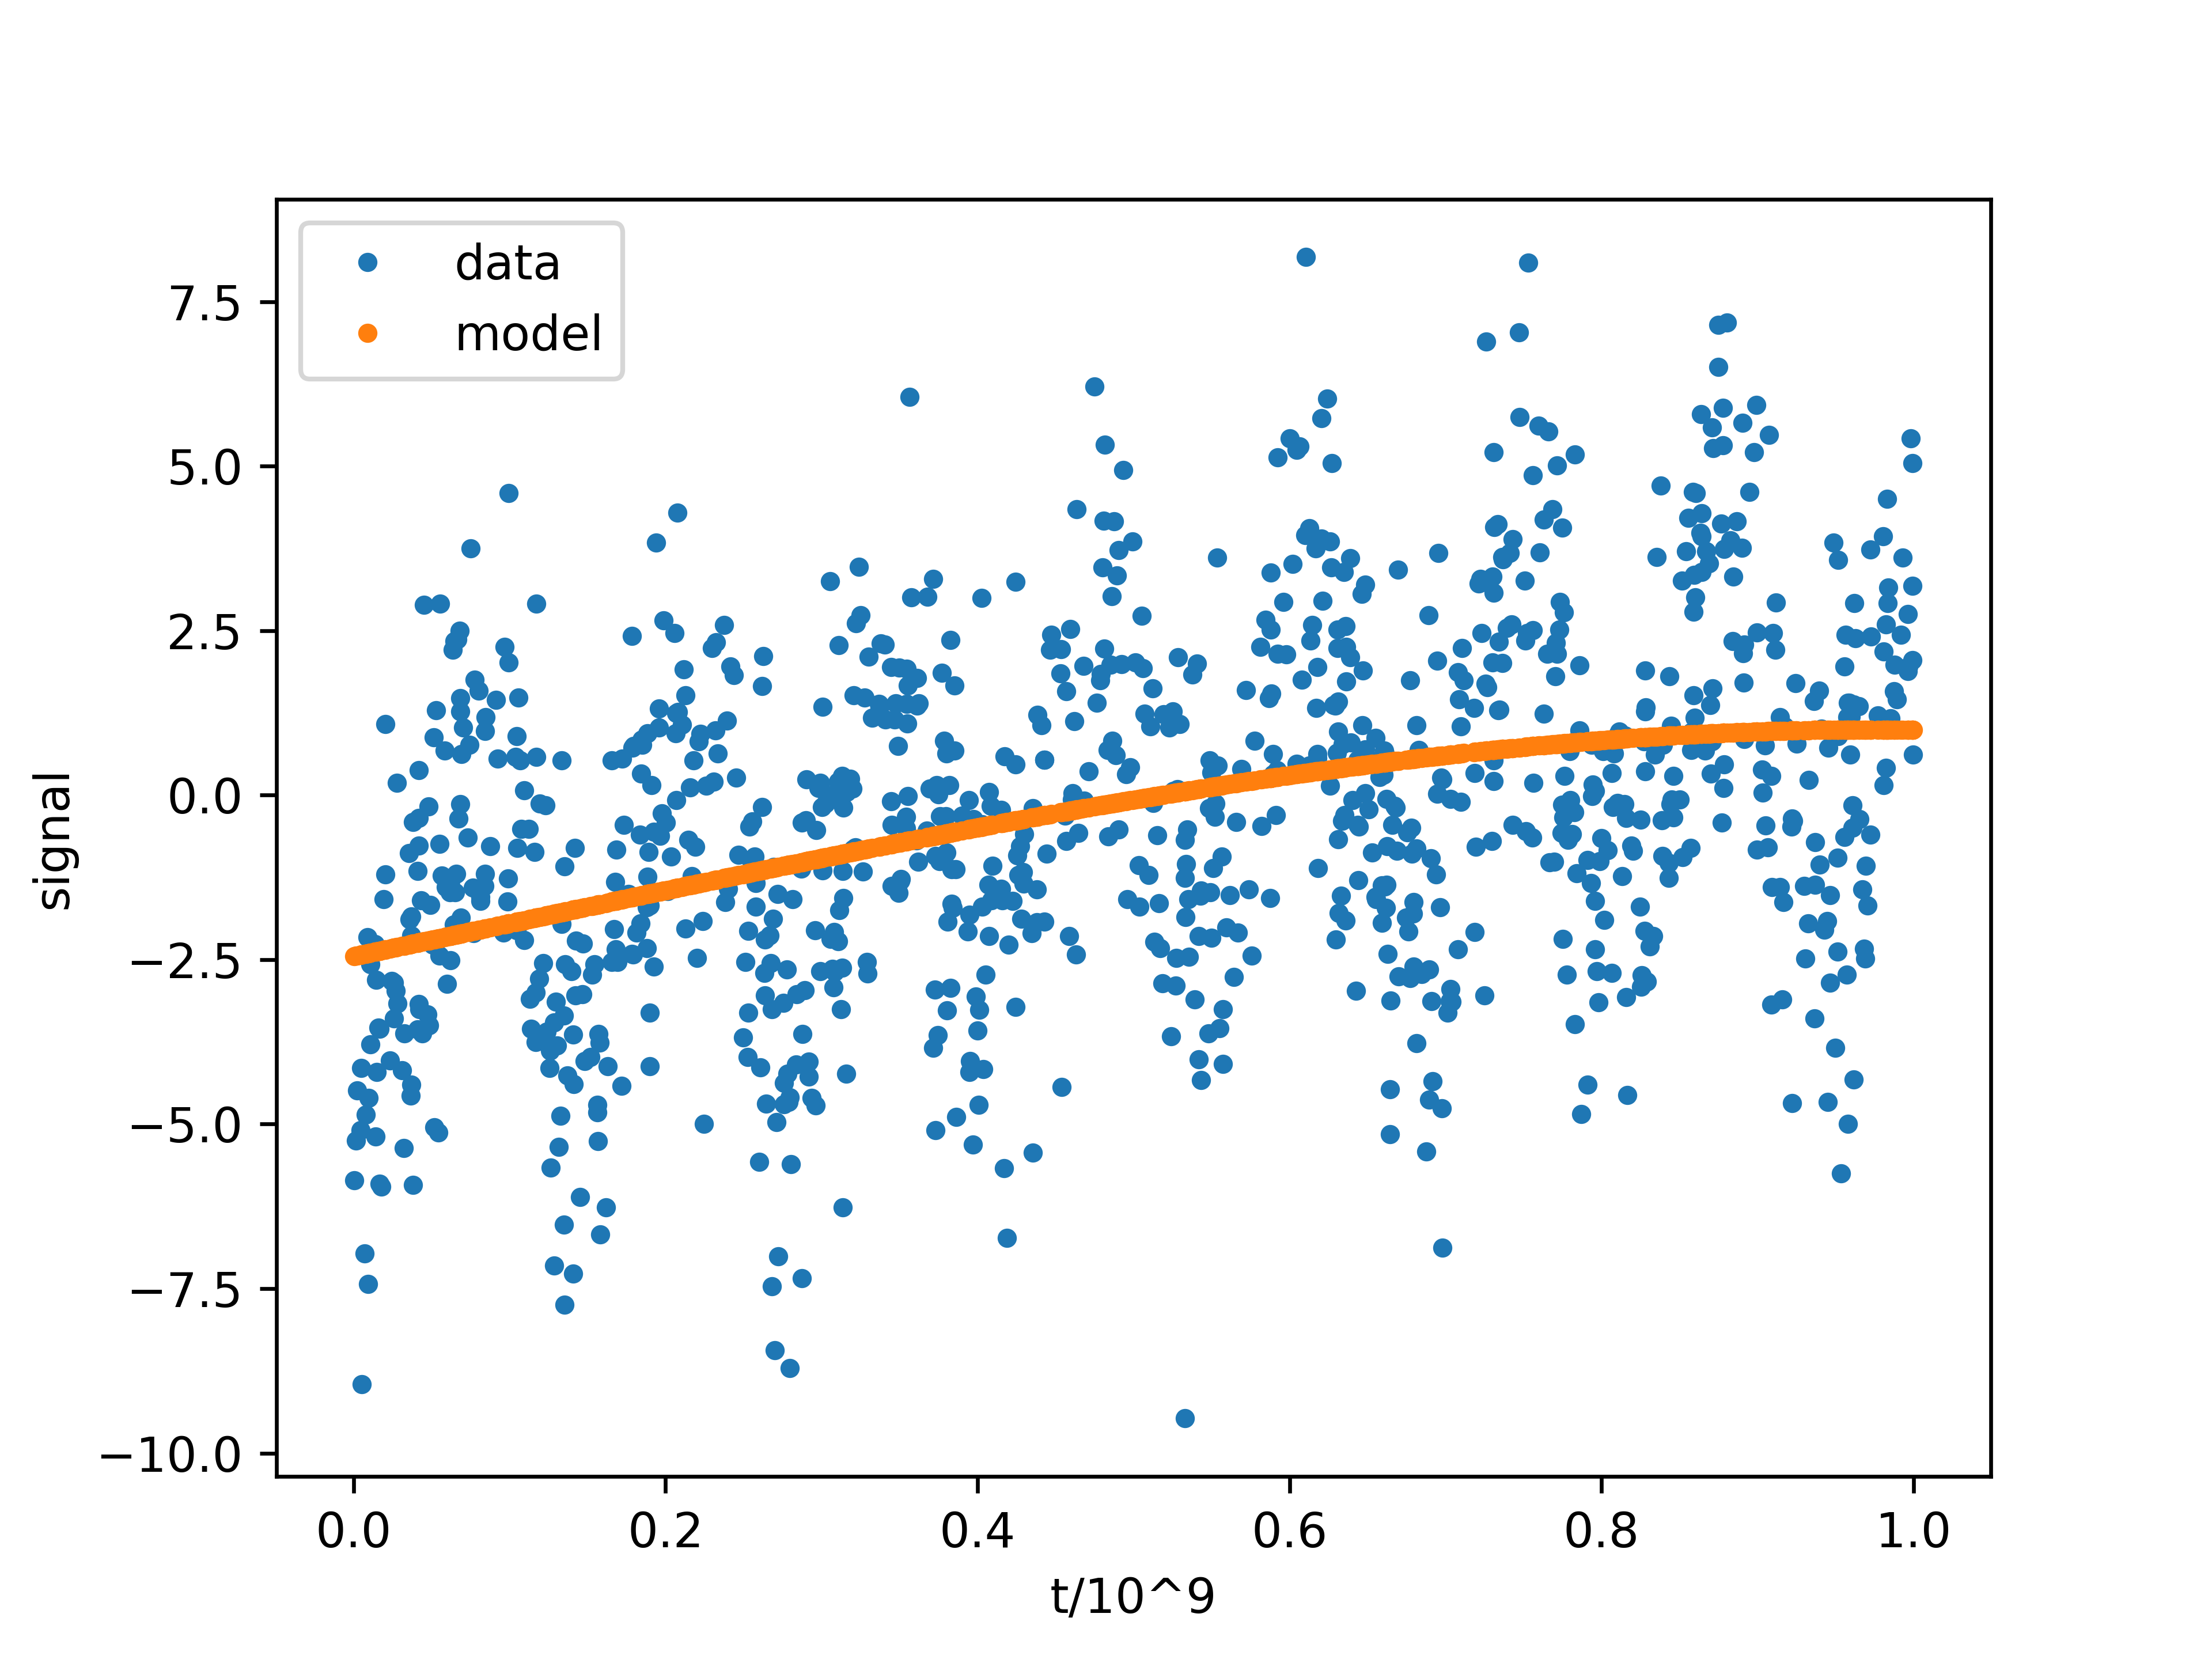
\includegraphics[width=12cm]{ps5-3-2.png}
\end{table}%

Then we calculated the residual of our observation data. We especially calculated the number of observation data being inside one sigma of uncertainty. We found that there's only 0.573 portion of the data inside one sigma, which is significantly lower than the expected portion of 0.68 by gaussian distribution. We think that this cannot satisfies us.

We then attempt to fit the data with 10th-order polynomial and 20th-order polynomial. Here's our fitted result:

\begin{table}[!h]
    \centering
    \caption{Fitted signal data to 10th-order polynomial}
    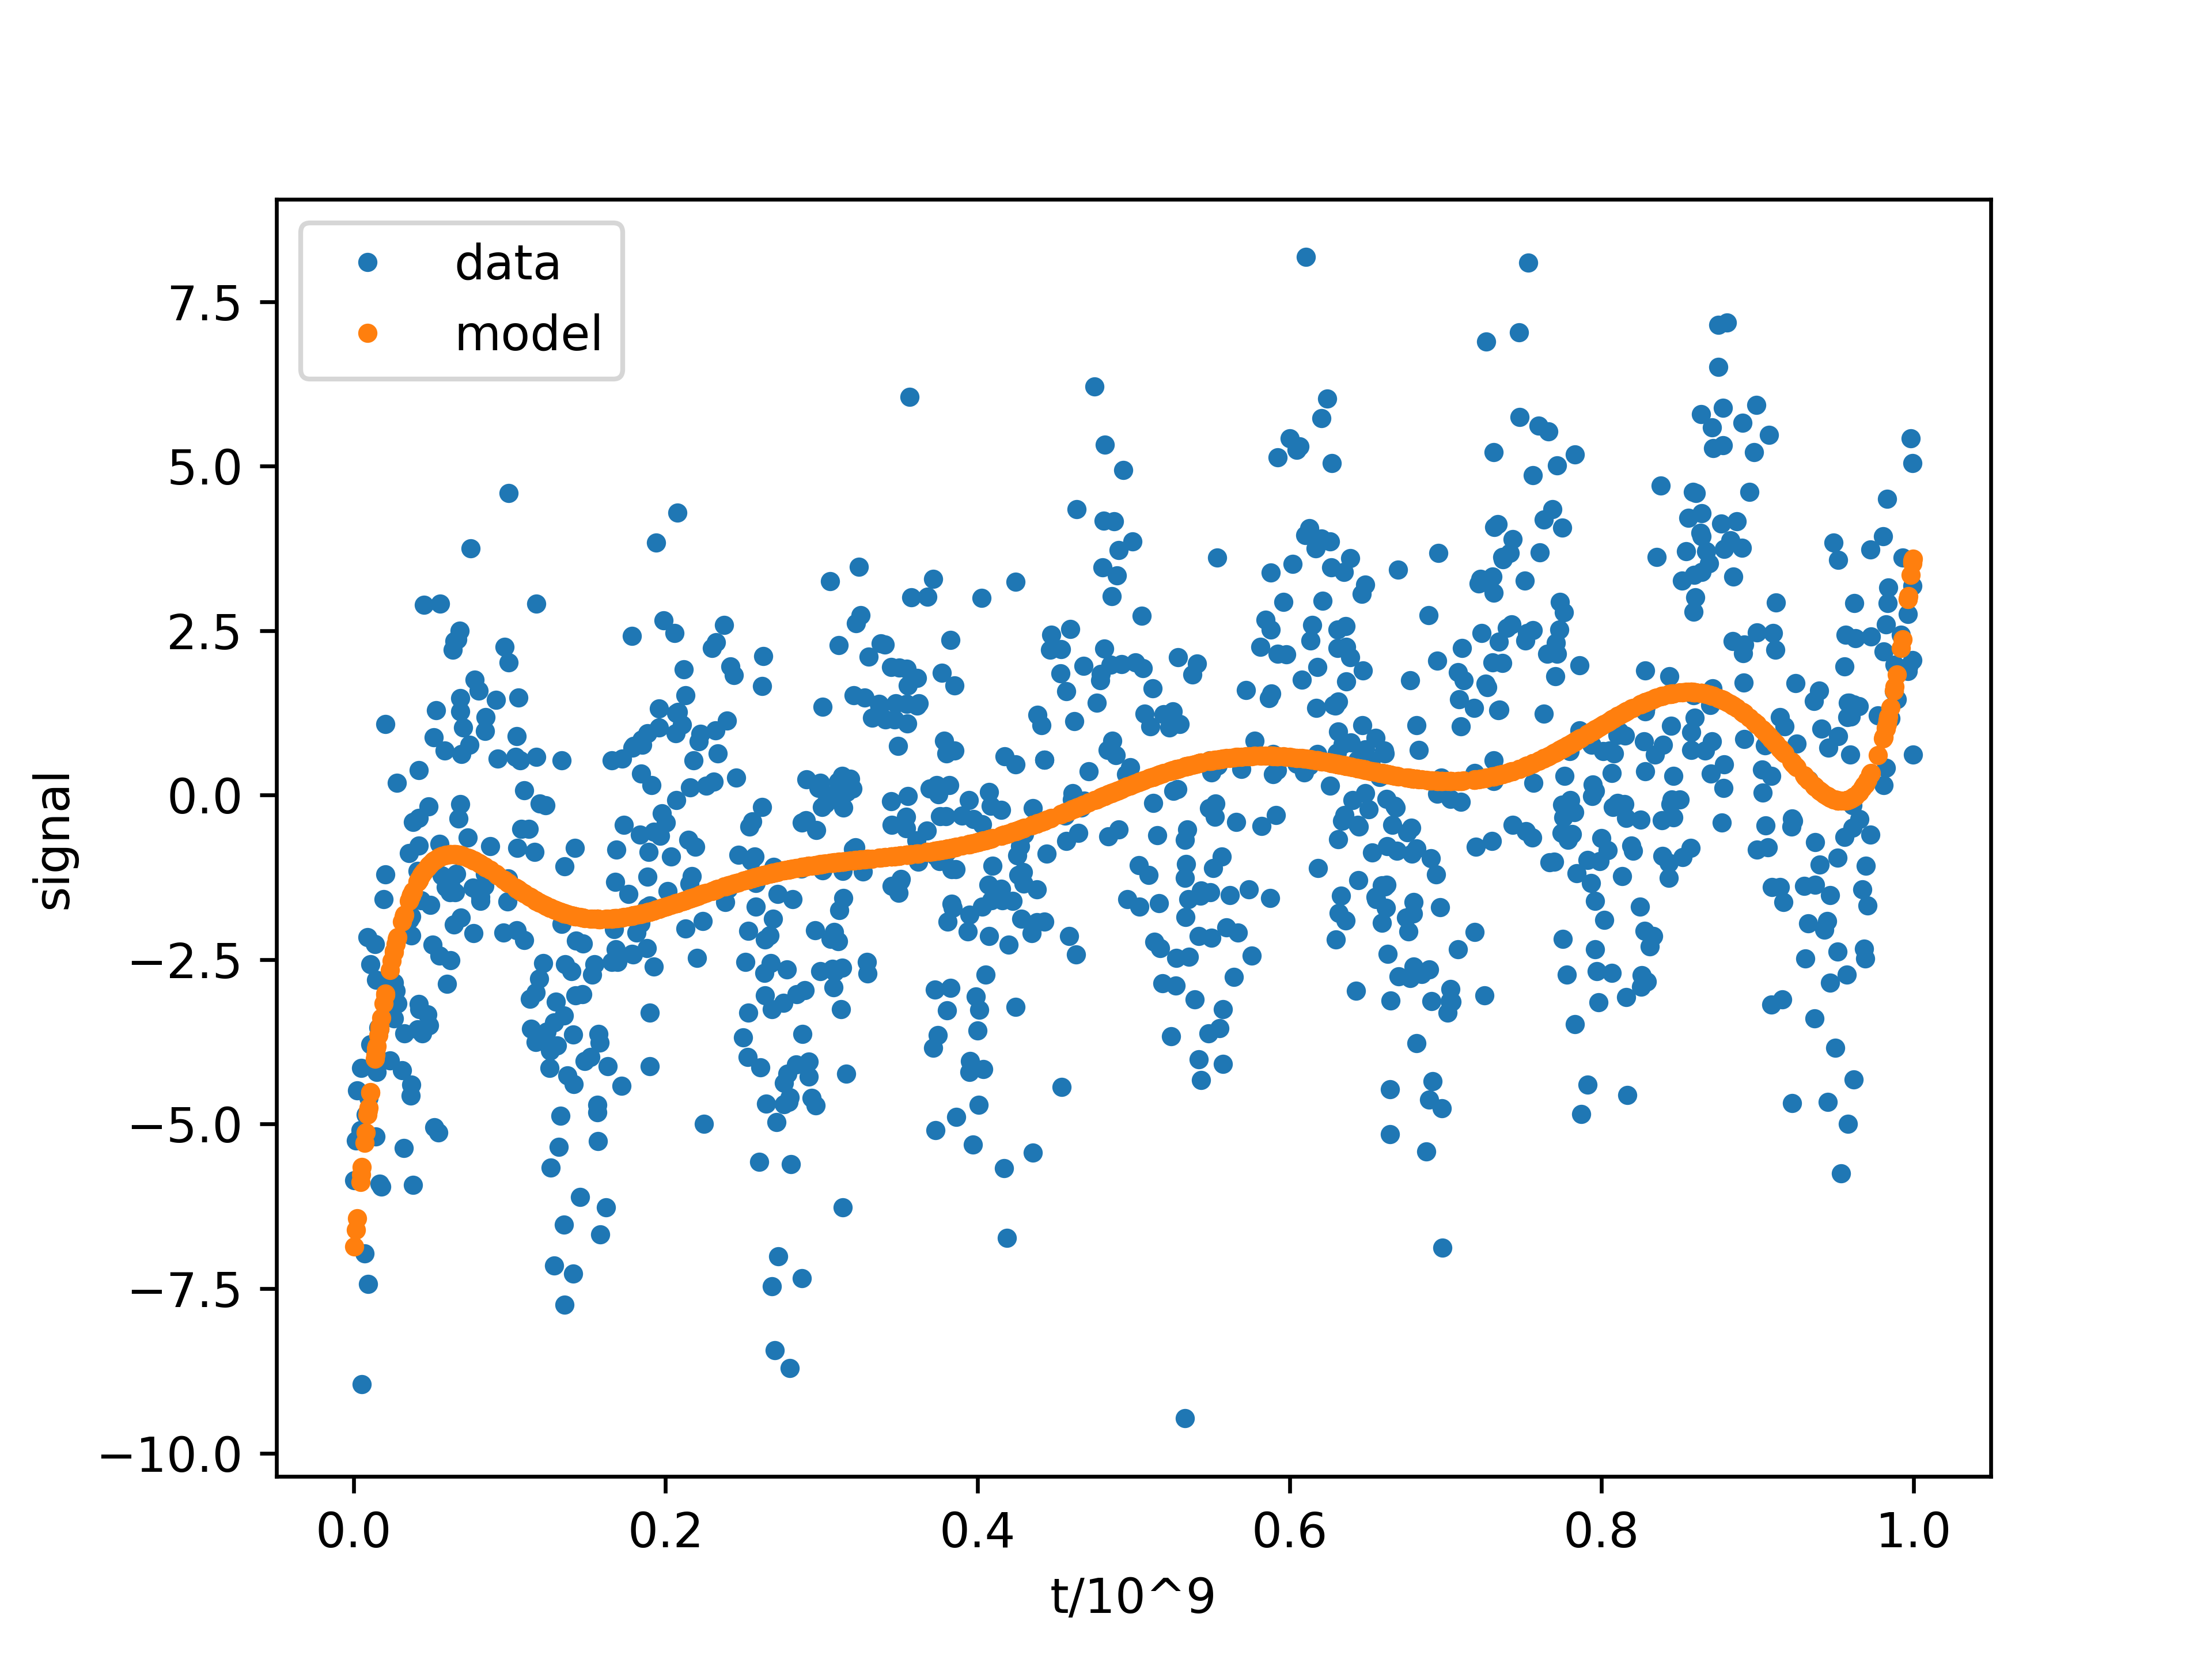
\includegraphics[width=11cm]{ps5-3-4-10.png}
\end{table}%

\begin{table}[!h]
    \centering
    \caption{Fitted signal data to 20th-order polynomial}
    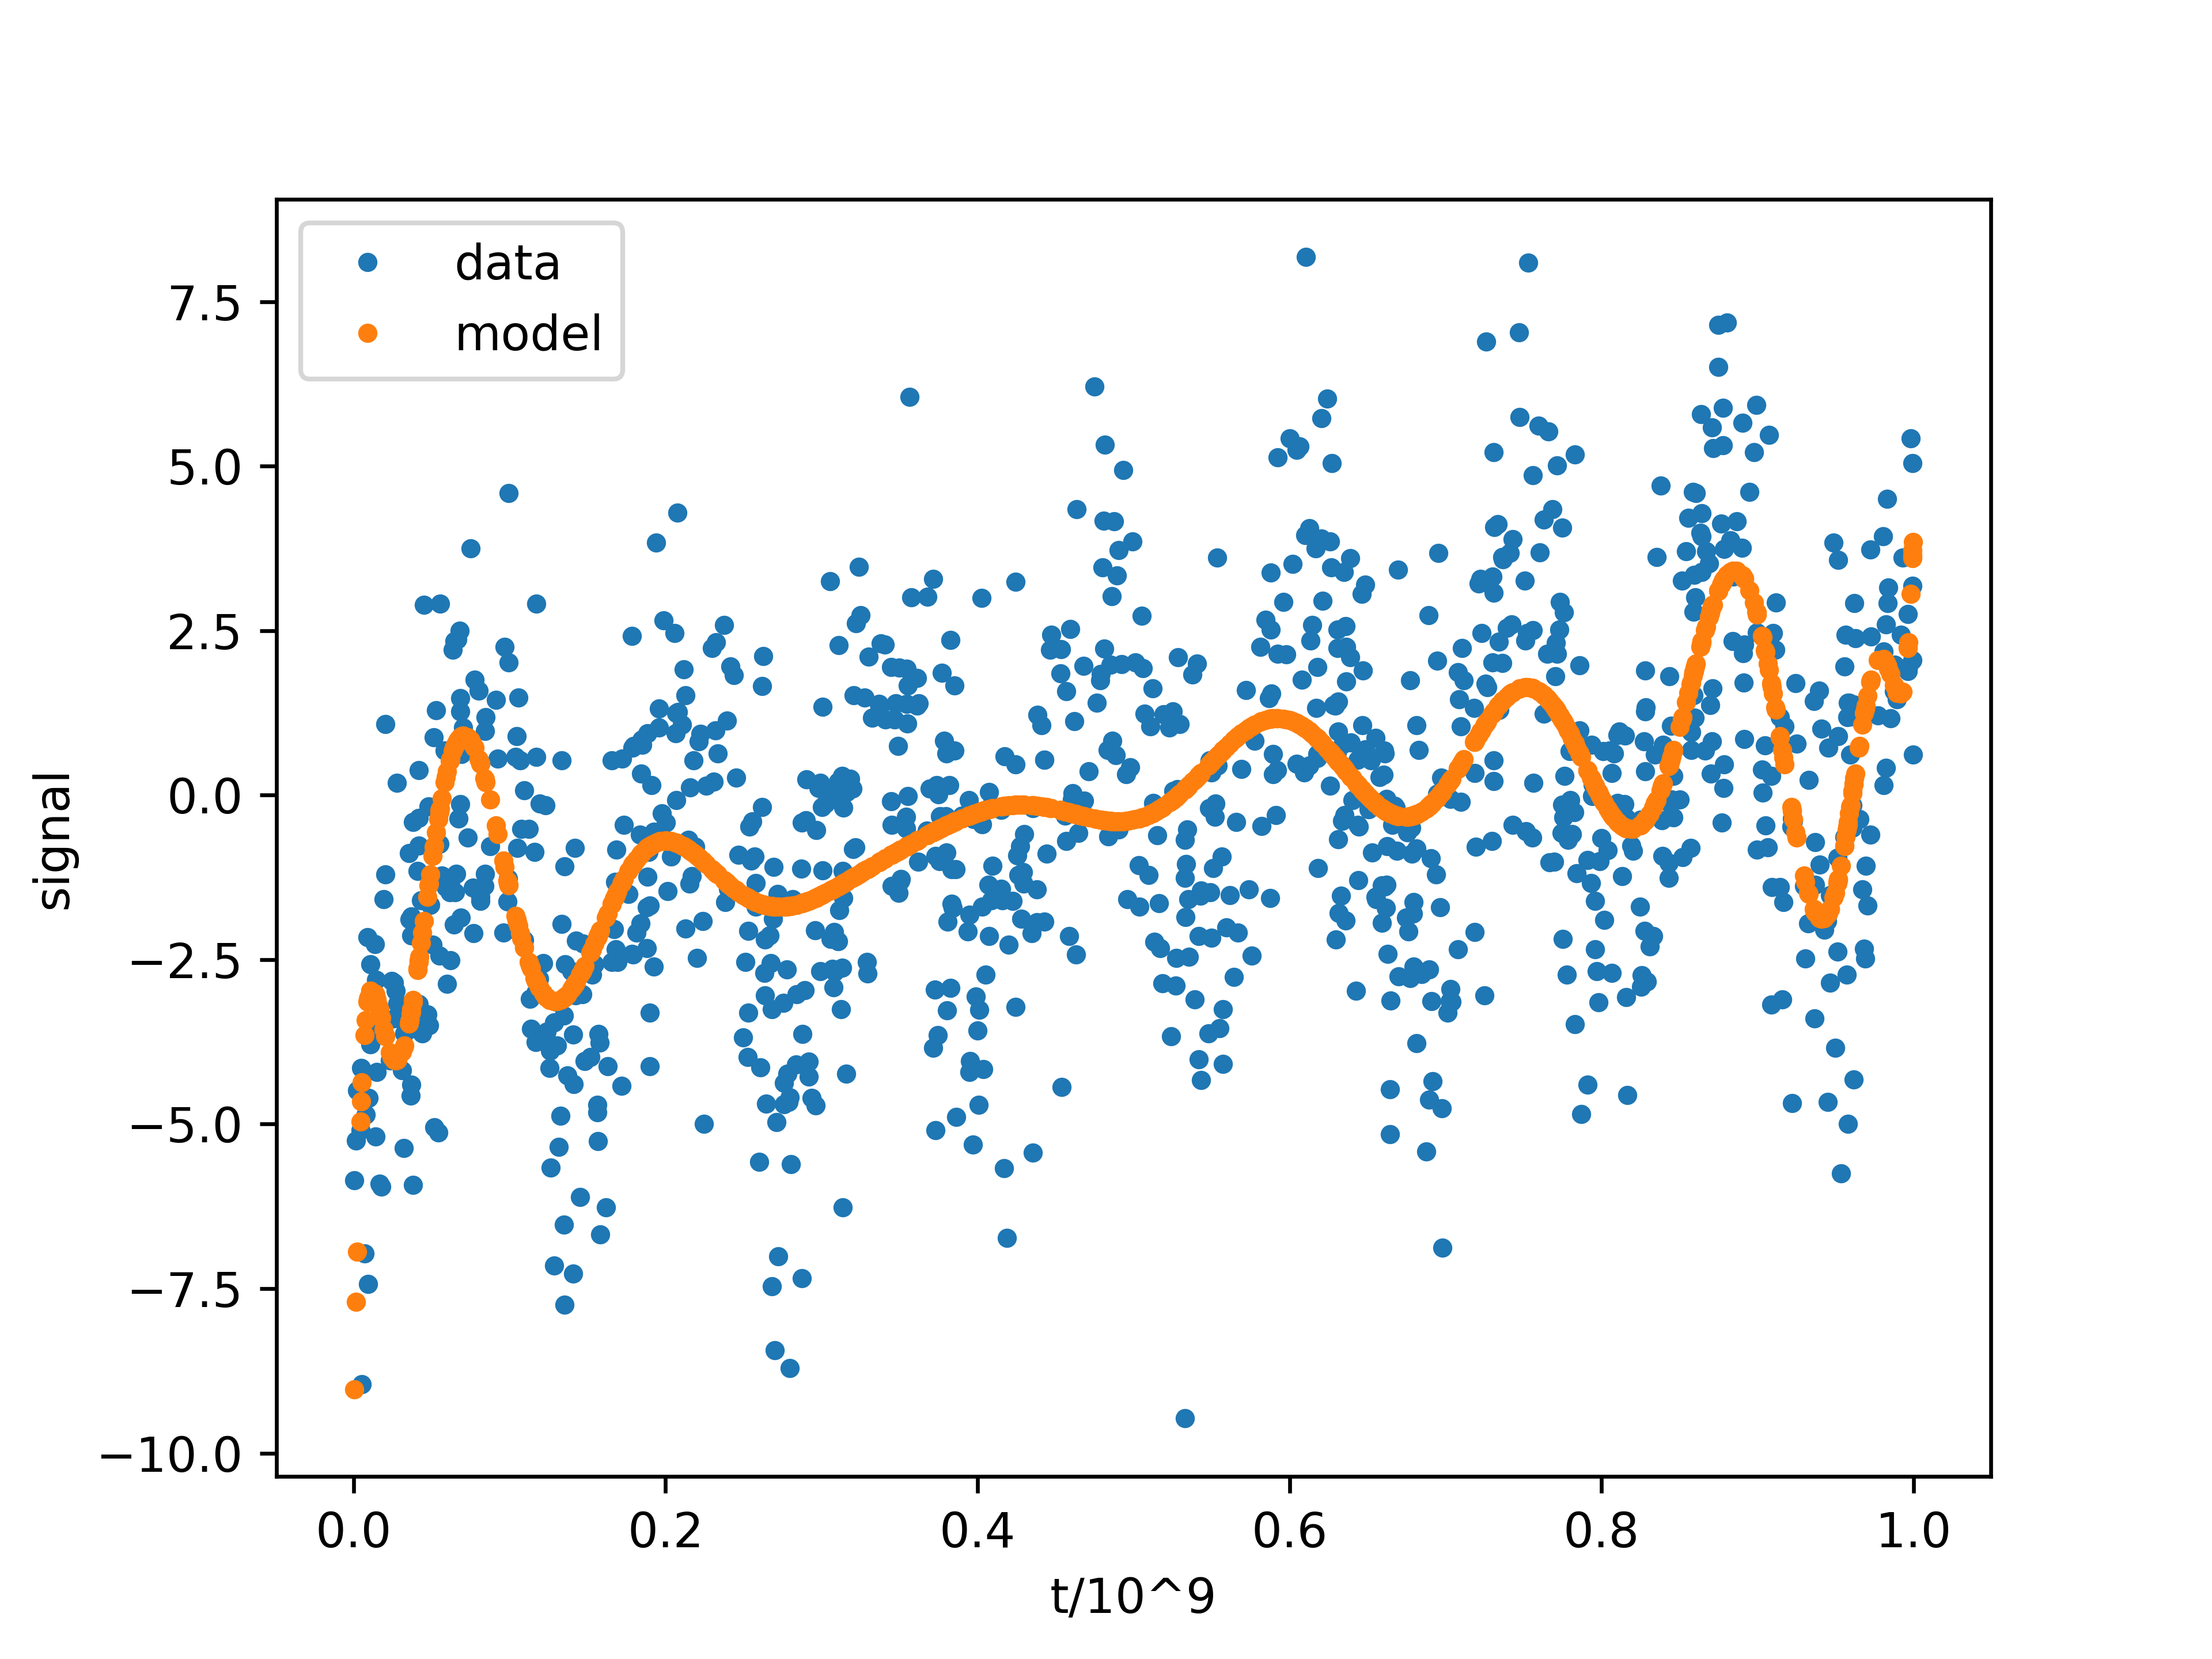
\includegraphics[width=11cm]{ps5-3-4-20.png}
\end{table}%

\newpage

The condition number is respectively 3898066.283726428(10th order) and 154815469309063.1(20th order). We found that the fitted result is not good enough and the condition number has become insanely big.

Finally we tried to fit the data with function with routine(doing fourier decomposition). We fit our data with sine and cosine function with frequency from 3.0 to 8.0, with step of 0.25. Here's our fitted result:

\begin{table}[!h]
    \centering
    \caption{Fitted signal data to routine functions}
    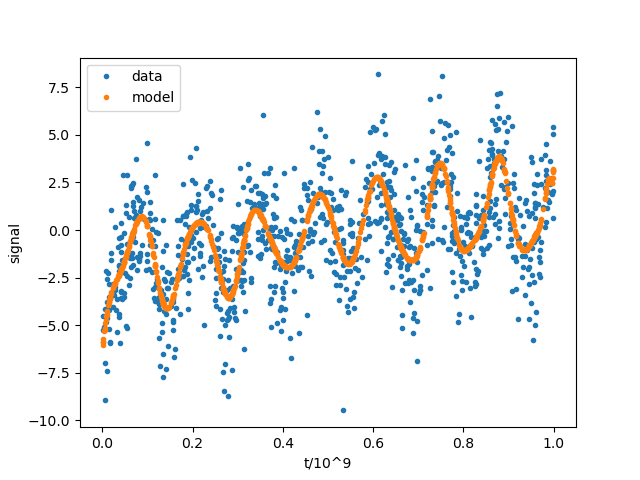
\includegraphics[width=12cm]{ps5-3-55.png}
\end{table}%

We found that this fitting result lead to 0.694 of all datas inside one sigma for theoretical prediction, which is close to theoretical result of 0.683 for gaussian distribution. This implies that our model is doing a quite good job explaining the observation data. We can actually look at the fitted diagram or go back to find the maximum value of singular value inside W to see that the principal frequency is around 7.5($*10^9$)
  







\end{document}